% A rotation by theta about the axis u: the vector v is turned to q v q^{-1}, with q = cos(theta/2) + sin(theta/2) u. Oblique projection. Generated by a short script.
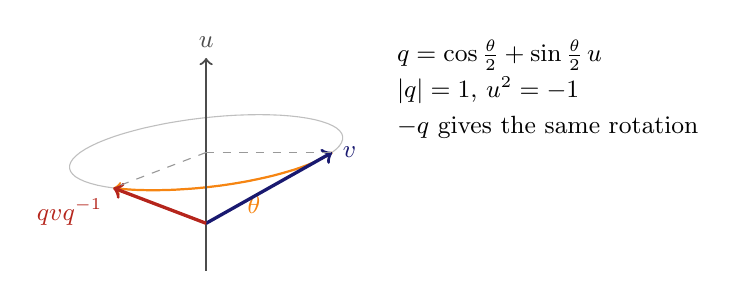
\begin{tikzpicture}[font=\small]
\draw[black!25] (1.600,0.900) -- (1.535,0.858) -- (1.459,0.817) -- (1.372,0.776) -- (1.274,0.736) -- (1.166,0.697) -- (1.050,0.660) -- (0.925,0.625) -- (0.794,0.591) -- (0.656,0.561) -- (0.514,0.532) -- (0.367,0.507) -- (0.218,0.484) -- (0.067,0.465) -- (-0.084,0.449) -- (-0.235,0.436) -- (-0.384,0.427) -- (-0.530,0.422) -- (-0.672,0.420) -- (-0.809,0.422) -- (-0.940,0.427) -- (-1.063,0.436) -- (-1.179,0.449) -- (-1.285,0.465) -- (-1.382,0.484) -- (-1.468,0.507) -- (-1.543,0.532) -- (-1.607,0.561) -- (-1.658,0.591) -- (-1.696,0.625) -- (-1.722,0.660) -- (-1.734,0.697) -- (-1.733,0.736) -- (-1.719,0.776) -- (-1.692,0.817) -- (-1.652,0.858) -- (-1.600,0.900) -- (-1.535,0.942) -- (-1.459,0.983) -- (-1.372,1.024) -- (-1.274,1.064) -- (-1.166,1.103) -- (-1.050,1.140) -- (-0.925,1.175) -- (-0.794,1.209) -- (-0.656,1.239) -- (-0.514,1.268) -- (-0.367,1.293) -- (-0.218,1.316) -- (-0.067,1.335) -- (0.084,1.351) -- (0.235,1.364) -- (0.384,1.373) -- (0.530,1.378) -- (0.672,1.380) -- (0.809,1.378) -- (0.940,1.373) -- (1.063,1.364) -- (1.179,1.351) -- (1.285,1.335) -- (1.382,1.316) -- (1.468,1.293) -- (1.543,1.268) -- (1.607,1.239) -- (1.658,1.209) -- (1.696,1.175) -- (1.722,1.140) -- (1.734,1.103) -- (1.733,1.064) -- (1.719,1.024) -- (1.692,0.983) -- (1.652,0.942) -- (1.600,0.900) -- cycle;
\draw[->,BurntOrange,thick] (1.600,0.900) -- (1.552,0.868) -- (1.497,0.837) -- (1.436,0.805) -- (1.368,0.774) -- (1.295,0.744) -- (1.215,0.714) -- (1.131,0.685) -- (1.041,0.658) -- (0.947,0.631) -- (0.849,0.605) -- (0.747,0.581) -- (0.642,0.558) -- (0.534,0.536) -- (0.423,0.516) -- (0.311,0.498) -- (0.197,0.481) -- (0.083,0.467) -- (-0.032,0.454) -- (-0.147,0.443) -- (-0.261,0.435) -- (-0.374,0.428) -- (-0.485,0.423) -- (-0.594,0.421) -- (-0.701,0.420) -- (-0.804,0.422) -- (-0.904,0.425) -- (-1.000,0.431) -- (-1.092,0.439) -- (-1.179,0.449);
\node[text=BurntOrange,below right] at (0.402,0.470) {$\theta$};
\draw[->,black!70,thick] (0.000,-0.600) -- (0.000,2.100) node[above] {$u$};
\draw[->,MidnightBlue,very thick] (0.000,0.000) -- (1.600,0.900) node[right] {$v$};
\draw[->,BrickRed,very thick] (0.000,0.000) -- (-1.179,0.449) node[below left] {$qvq^{-1}$};
\draw[black!40,dashed] (0.000,0.900) -- (1.600,0.900);
\draw[black!40,dashed] (0.000,0.900) -- (-1.179,0.449);
\node[align=left,anchor=west,font=\small] at (2.3,1.7) {$q=\cos\frac\theta2+\sin\frac\theta2\,u$\\[2pt]$|q|=1$, $u^2=-1$\\[2pt]$-q$ gives the same rotation};
\end{tikzpicture}
